% Planning a Drone Swarm Sweep over a Field of Any Shape
% Team Asclepius, NIDAR Rescueswarm
%
% Overleaf: create a new project, paste this file as main.tex, and upload the
% four PNGs from paper/figures/ into a folder named "figures".
% Compiles with pdfLaTeX.

\documentclass[11pt,a4paper]{article}

\usepackage[T1]{fontenc}
\usepackage[utf8]{inputenc}
\usepackage{lmodern}
\usepackage[margin=2.5cm]{geometry}
\usepackage{amsmath,amssymb,amsthm}
\usepackage{graphicx}
\usepackage{booktabs}
\usepackage{array}
\usepackage{enumitem}
\usepackage{caption}
\usepackage[authoryear,round]{natbib}
\usepackage{xcolor}
\usepackage[colorlinks=true,linkcolor=blue!50!black,citecolor=blue!50!black,urlcolor=blue!50!black]{hyperref}

\captionsetup{font=small,labelfont=bf}
\setlist{itemsep=2pt,topsep=4pt}
\newtheorem{proposition}{Proposition}

\newcommand{\dd}{\mathrm{d}}
\newcommand{\HFOV}{\mathrm{HFOV}}
\newcommand{\VFOV}{\mathrm{VFOV}}

\title{Planning a Drone Swarm Sweep over a Field of Any Shape}
\author{Team Asclepius, NIDAR Rescueswarm}
\date{October 2026}

\begin{document}
\maketitle

\begin{abstract}
A line of drones flies over a field and photographs it with downward-pointing cameras. Each drone can fly higher to see a wider strip of ground. We want every point of the field photographed, using altitudes that are as low as possible.

We first look for one \emph{centre line} through the field such that, wherever the drones are, the line cuts their row exactly in half. Writing this as a calculus-of-variations problem with a Lagrangian and deriving its equations shows three things. First, the equations reduce to a single direction field, so the centre line is fixed once its starting point on the boundary is chosen. Second, such a line always exists in convex fields. Third, in strongly non-convex fields the traced line usually circles forever and never reaches the other side, which explains why our first numerical solver failed.

We therefore relax the problem. Instead of one centre line, the sweep is described by a \emph{time map} giving, for every point, the moment the drone line passes over it. We compare four time maps. The \emph{harmonic} map, obtained by minimising an energy, needed the lowest altitude on every field we tested. Finally, we divide the field among the drones and set their altitudes so that the whole field is photographed, and this coverage is guaranteed.
\end{abstract}

\noindent\textbf{Code:} \url{https://github.com/Avinashistoocool/asclepius} (folder \texttt{swarm\_lab}).\\
\textbf{Interactive demo:} \url{https://avinashistoocool.github.io/asclepius/}.\\
\textbf{Reproduction scripts:} \texttt{paper/verify\_derivations.py}, \texttt{paper/figures.py}, \texttt{paper/results.py}.

%==========================================================================
\section{The problem}
%==========================================================================

\begin{itemize}
  \item \textbf{Field.} A region $\Omega$ in the plane bounded by a closed curve. In the code it is a polygon on a $600\times600$ canvas; all distances are in canvas units.
  \item \textbf{Swarm.} $N$ drones flying side by side as a flexible line. The line may bend, and it may split into groups to pass around an obstacle and rejoin later.
  \item \textbf{Camera.} Each drone carries a downward (\emph{nadir}) camera with horizontal and vertical fields of view $\HFOV$ and $\VFOV$. At altitude $h$ it photographs a rectangle of width $2h\tan(\HFOV/2)$ and length $2h\tan(\VFOV/2)$, centred under the drone and turned to its direction of travel.
  \item \textbf{Goal.} Every point of the field appears in at least one photo, with the highest altitude kept low, paths kept short, and work shared evenly among the drones.
\end{itemize}

This is a \emph{coverage path planning} problem \citep{choset2001,galceran2013,cabreira2019}. Most existing methods either sweep with straight back-and-forth passes \citep{choset1998} or divide the field into one region per robot \citep{cortes2004}. Our case differs because the drones fly together as a single line, and because each drone chooses its own altitude.

%==========================================================================
\section{First idea: a centre line that cuts every chord in half}
%==========================================================================

\subsection{What we were looking for}

Think of the drones as a straight row moving forward. The row is a \textbf{chord} of the field: a straight segment with both ends on the boundary. Suppose the row is always perpendicular to a smooth curve $p(s)$ and centred on it. Then $p(s)$ is the path of the middle drone, and the row reaches equally far to both sides.

\begin{figure}[ht]
  \centering
  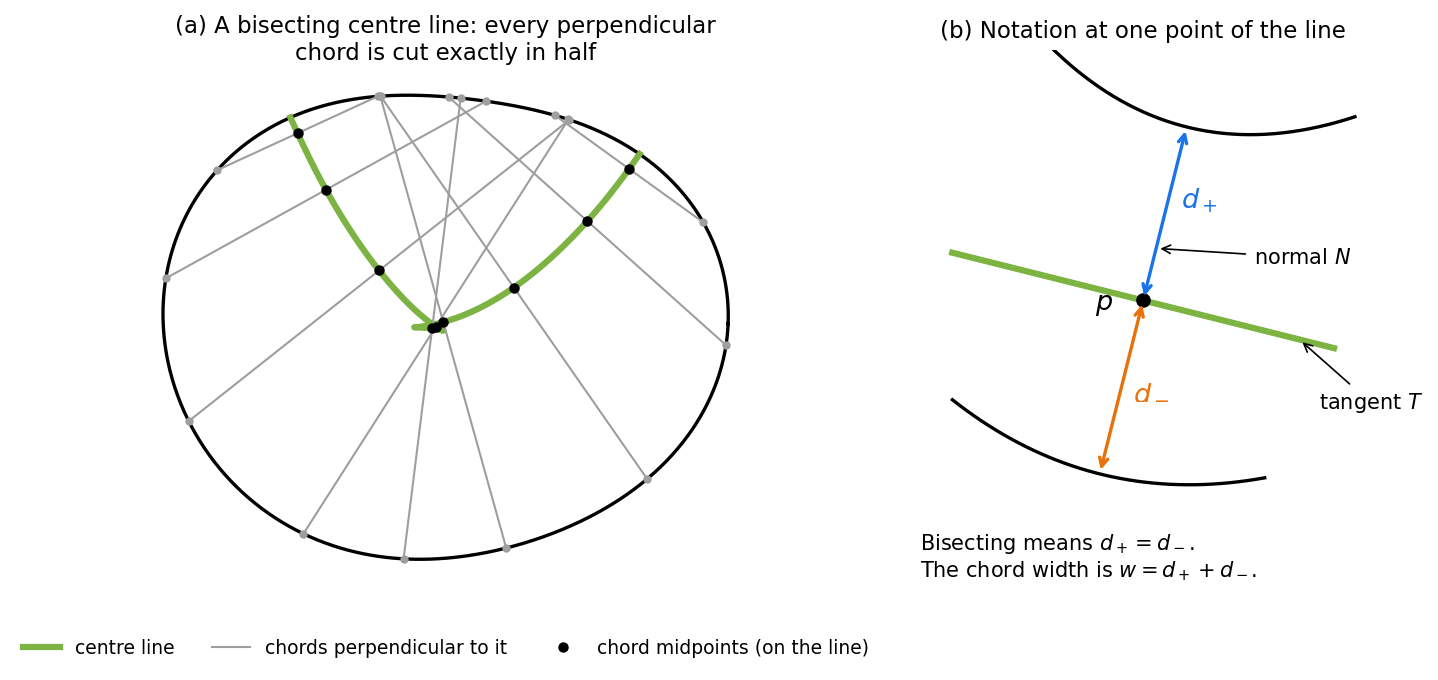
\includegraphics[width=\textwidth]{figures/fig1_bisecting.png}
  \caption{(a) A centre line (green) through a convex field. Each grey chord is perpendicular to the line, and its midpoint (black dot) lies on the line. (b) The quantities used at one point: $T$ is the direction of the line, $N$ is perpendicular to it, and $d_+$, $d_-$ are the distances to the boundary on each side.}
  \label{fig:bisecting}
\end{figure}

\paragraph{Notation.} At a point $p$ on the line:

\begin{center}
\begin{tabular}{>{$}l<{$} l}
\toprule
\text{Symbol} & Meaning \\
\midrule
s & distance travelled along the line \\
T,\ N & unit direction of the line, and the unit vector perpendicular to it \\
\theta & angle of $N$ \\
d_+,\ d_- & distance from $p$ to the first boundary point hit along $+N$ and along $-N$ \\
w = d_+ + d_- & chord width (length of the drone row) \\
e = \tfrac12(d_+ - d_-) & distance from $p$ to the chord's midpoint (zero when the chord is bisected) \\
\kappa & curvature of the line: how fast $T$ turns per unit length \\
\bottomrule
\end{tabular}
\end{center}

\noindent The requirement is $e=0$ everywhere along the line, that is, $d_+ = d_-$.

\subsection{Why this is the right requirement: the swept-area formula}

When the row moves a short distance $\dd s$ along the line, it sweeps a thin strip of area $\dd A$. A drone at signed offset $r$ from the centre travels $(1-\kappa r)\,\dd s$, since drones on the inside of a bend move less. Summing over the row,
\begin{equation}
\frac{\dd A}{\dd s} = \int_{-d_-}^{d_+} (1-\kappa r)\,\dd r = w\,(1-\kappa e).
\label{eq:area}
\end{equation}

\begin{itemize}
  \item When $e=0$, the swept area is exactly $\int w\,\dd s$, with no correction for curvature. This is why a bisecting line is desirable.
  \item The row only moves forward if no drone travels backwards, which requires
  \begin{equation}
  \kappa\,d_+ < 1 \quad\text{and}\quad -\kappa\,d_- < 1.
  \label{eq:nofold}
  \end{equation}
  In words: in a bend, the inner end of the row must not pass the centre of the bend. If \eqref{eq:nofold} fails, consecutive chords cross and the row \textbf{folds} over itself.
\end{itemize}

\subsection{Writing it as a Lagrangian}

To choose the \emph{best} centre line, we minimise a cost $\int f\,\dd s$ along it, where $f$ may depend on the position $p$ and the direction $\theta$. A natural choice is $f=w$, the chord width, which by \eqref{eq:area} equals the swept area. The Lagrangian is
\begin{equation}
\mathcal{L} = f(p,\theta)\,|p'|.
\label{eq:lagrangian}
\end{equation}
The factor $|p'|$ makes the cost independent of how fast the line is traversed. The Euler--Lagrange equation of \eqref{eq:lagrangian} \citep{gelfand1963} reduces to a single equation for the curvature:
\begin{equation}
\kappa\,\bigl(f + f_{\theta\theta}\bigr) = \partial_N f - \partial_T f_\theta .
\label{eq:el}
\end{equation}
Here $f_\theta$ and $f_{\theta\theta}$ are derivatives with respect to the direction, and $\partial_N$, $\partial_T$ are derivatives along $N$ and $T$.

\begin{itemize}
  \item If $f$ does not depend on the direction, \eqref{eq:el} becomes $\kappa f = \partial_N f$: the line bends towards cheaper regions, just as light bends in glass.
  \item The quantity $f+f_{\theta\theta}$ acts as the \emph{stiffness} of the line. Where it is negative, the equation has no smooth solution and the line develops corners. The same quantity appears in the theory of crystal shapes \citep{taylor1978,gurtin1993}.
\end{itemize}

Equation \eqref{eq:el} needs the derivatives of the wall distances $d_\pm$. Moving $p$ or turning the chord changes where the chord meets the wall. Let $n$ be the chord direction, $\alpha$ its angle, $n_\perp$ the chord direction turned by $90^\circ$, and $\nu$ the outward normal of the wall at the hit point. Then
\begin{equation}
\nabla_p d = -\frac{\nu}{\nu\cdot n}, \qquad
\frac{\partial d}{\partial\alpha} = -\,d\,\frac{\nu\cdot n_\perp}{\nu\cdot n}.
\label{eq:hit}
\end{equation}
Both expressions blow up when $\nu\cdot n\to0$, that is, when the chord \textbf{grazes} the wall. In a non-convex field the chord then jumps to a different part of the wall, and $d$ jumps with it. This turns out to be the root of the difficulty.

\subsection{The requirement fixes the line almost completely}

Adding the requirement $e=0$ through a Lagrange multiplier $\lambda(s)$ gives the constrained Lagrangian
\begin{equation}
\mathcal{L}_\lambda = \bigl(f + \lambda\,e\bigr)\,|p'| .
\label{eq:constrained}
\end{equation}
However, the requirement $e=0$ involves only the position $p$ and the direction $\theta$, not the rate at which the direction changes. So \textbf{at every point, $e=0$ already tells us which way the line must go}. It defines a direction field that the centre line must follow. The only free choice left is the boundary point $c$ where the line starts, and minimising cost reduces to a one-variable search:
\begin{equation}
\min_{c\ \in\ \partial\Omega}\ \int_{\text{line starting at } c} f\,\dd s .
\label{eq:search}
\end{equation}

\begin{proposition}[Existence of a bisecting direction]
Let $p$ be a point of $\Omega$, and suppose $d_\pm$ vary continuously as the chord through $p$ is rotated. This holds in particular when $\Omega$ is convex. Then some direction at $p$ gives $e=0$.
\end{proposition}
\begin{proof}
Rotating the chord by $180^\circ$ swaps its two ends, so $e$ changes sign. A continuous function that changes sign has a zero (intermediate value theorem).
\end{proof}

In a non-convex field, the jumps described after \eqref{eq:hit} can skip over zero, leaving no valid direction. They can also produce several zeros, so the line can branch.

\subsection{Why our first solver failed}

The first implementation represented the line as a smooth spline and adjusted it by least squares until $e\approx0$ at many sample points, with both ends pinned to the boundary. On most non-trivial fields it stopped with messages such as \texttt{Endpoint residual 0.0073; midpoint residual 3.648}, meaning the chord midpoints were still about 3.6 units off the line. The analysis above explains why:
\begin{enumerate}
  \item \textbf{The equations are not smooth.} $d_\pm$ jump when the chord switches wall segments, whereas least squares assumes smooth equations.
  \item \textbf{There are too many conditions.} By \eqref{eq:search} the line is fixed by its starting point, so pinning \emph{both} ends adds one condition too many. In general no solution exists.
  \item \textbf{The ends are degenerate.} At the boundary the chord shrinks to zero length, and the equations lose information there.
  \item \textbf{Sometimes no line exists at all} (Proposition~1 and Section~\ref{sec:tracing}).
\end{enumerate}

%==========================================================================
\section{Tracing the centre line directly}
\label{sec:tracing}
%==========================================================================

\subsection{Following the two chord ends instead of the midpoint}

Instead of moving the midpoint and casting rays to the walls, we move the \textbf{two ends of the chord along the boundary}. Let the boundary be the curve $\gamma(u)$, and put the chord ends at $a=\gamma(u)$ and $b=\gamma(v)$. The midpoint is $m=(a+b)/2$ and the chord vector is $q=b-a$.

The chord must stay perpendicular to the path of its midpoint. Since $m' = \tfrac12\bigl(\gamma'(u)\,u' + \gamma'(v)\,v'\bigr)$, this means
\[
q\cdot m' = 0 \iff \bigl(q\cdot\gamma'(u)\bigr)\,u' + \bigl(q\cdot\gamma'(v)\bigr)\,v' = 0,
\]
so the two ends must move in the ratio
\begin{equation}
(u',\,v') \;\propto\; \bigl(q\cdot\gamma'(v),\; -\,q\cdot\gamma'(u)\bigr).
\label{eq:pair}
\end{equation}
This is an ordinary differential equation for $(u,v)$. It needs no ray casting and remains smooth as long as the boundary is smooth. Similar constructions from pairs of boundary points appear in shape analysis \citep{brady1984,leyton1987}.

\paragraph{Starting the trace.} At the start, both chord ends sit at the same boundary point $c$, giving a chord of length zero. Equation \eqref{eq:pair} is degenerate there, because both components vanish. Writing $u=c-d$ and $v=c+d$ and expanding for small $d$ gives
\begin{equation}
c' \approx -\,d\,\bigl(\gamma'\cdot\gamma''\bigr), \qquad d' \approx |\gamma'|^2,
\label{eq:start}
\end{equation}
which is perfectly regular. Hence \textbf{exactly one centre line starts from every boundary point}, and it leaves the boundary at a right angle. Starting from $c$ turns the problem into a step-by-step integration (an initial-value problem), as \eqref{eq:search} anticipated.

\paragraph{Chords where the line stops.} The chord stops moving when both terms in \eqref{eq:pair} vanish, which happens when the chord is perpendicular to the boundary at \emph{both} ends. Every smooth convex field has at least two such chords: the longest chord (the diameter) and the chord across the narrowest width.

\subsection{What happens in practice}

We integrated \eqref{eq:pair}--\eqref{eq:start} with a fourth-order Runge--Kutta method \citep{hairer1993} from 8 evenly spaced starting points on two smooth fields (Figure~\ref{fig:tracing}).

\begin{figure}[ht]
  \centering
  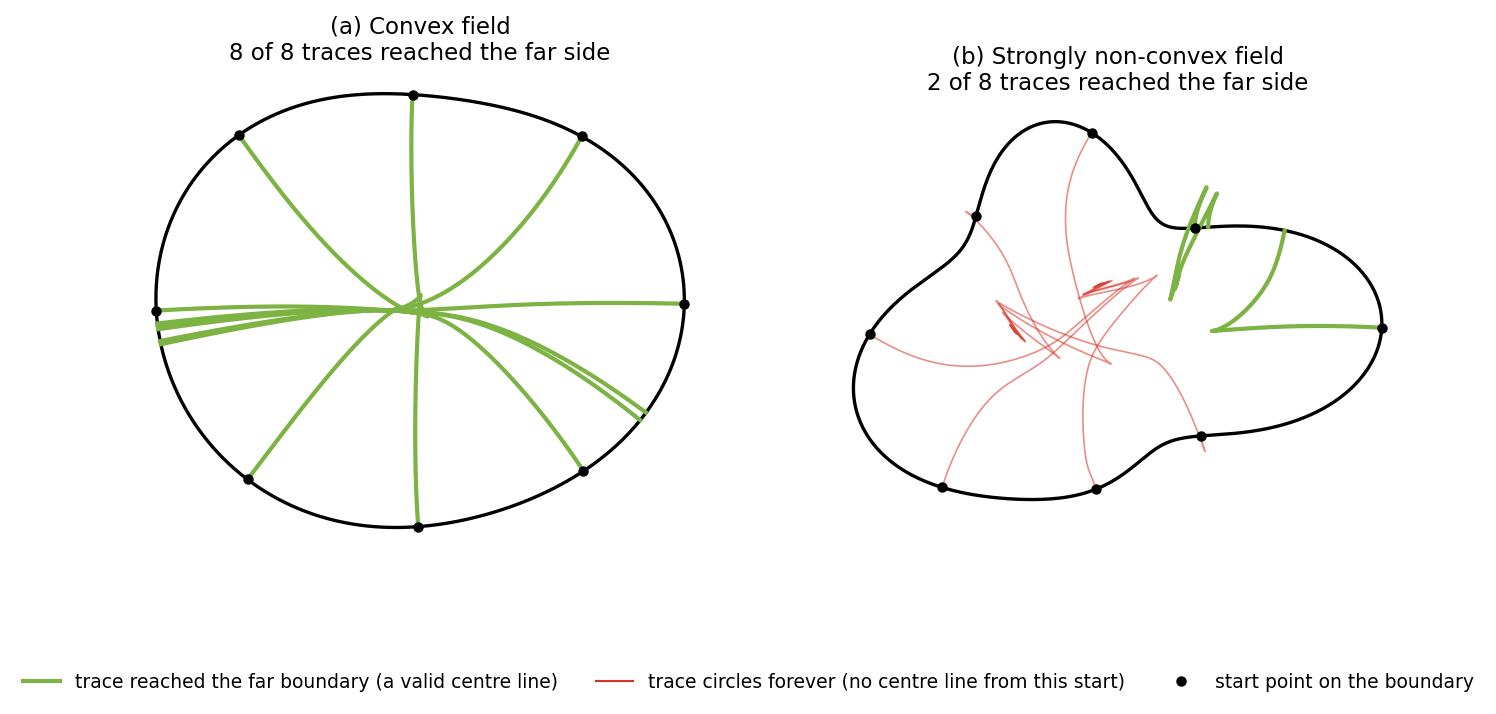
\includegraphics[width=\textwidth]{figures/fig2_tracing.png}
  \caption{Centre lines traced from 8 starting points (black dots). (a) In a convex field, all 8 traces cross the field and end on the opposite boundary, so each is a valid centre line. (b) In a strongly non-convex field, only 2 of the 8 reach the far side. The other 6 (red) keep circling inside the field, because the chord rotates without ever closing.}
  \label{fig:tracing}
\end{figure}

\paragraph{Conclusion.} Bisecting centre lines exist reliably only in convex or nearly convex fields. General fields need a different approach.

%==========================================================================
\section{The practical approach: a time map}
%==========================================================================

\subsection{The idea}

We drop the single centre line. Instead, the sweep is described by a \textbf{time map} $T(x)$, which gives for each point $x$ of the field the moment $0\le T\le1$ at which the drone line passes over it. At time $t$, the drone line is the curve on which $T(x)=t$, a \emph{level line} of the map.

\begin{itemize}
  \item Every point gets a time, so the whole field is swept by construction.
  \item If a level line breaks into several pieces, the swarm splits into groups.
  \item With $N$ drones spread evenly along a level line of length $\ell$, each drone covers a strip of width $\ell/N$. That width sets its altitude.
\end{itemize}

The coarea formula \citep{evans2010} links the time map to the length of the drone line:
\begin{equation}
\int_0^1 \bigl(\text{length of the drone line at time } t\bigr)\,\dd t = \int_\Omega |\nabla T|\,\dd x .
\label{eq:coarea}
\end{equation}
Keeping $|\nabla T|$ small therefore keeps the drone line short, and so keeps altitudes low. Each of our four planners is one choice of $T$ (Figure~\ref{fig:sweeps}).

\begin{figure}[ht]
  \centering
  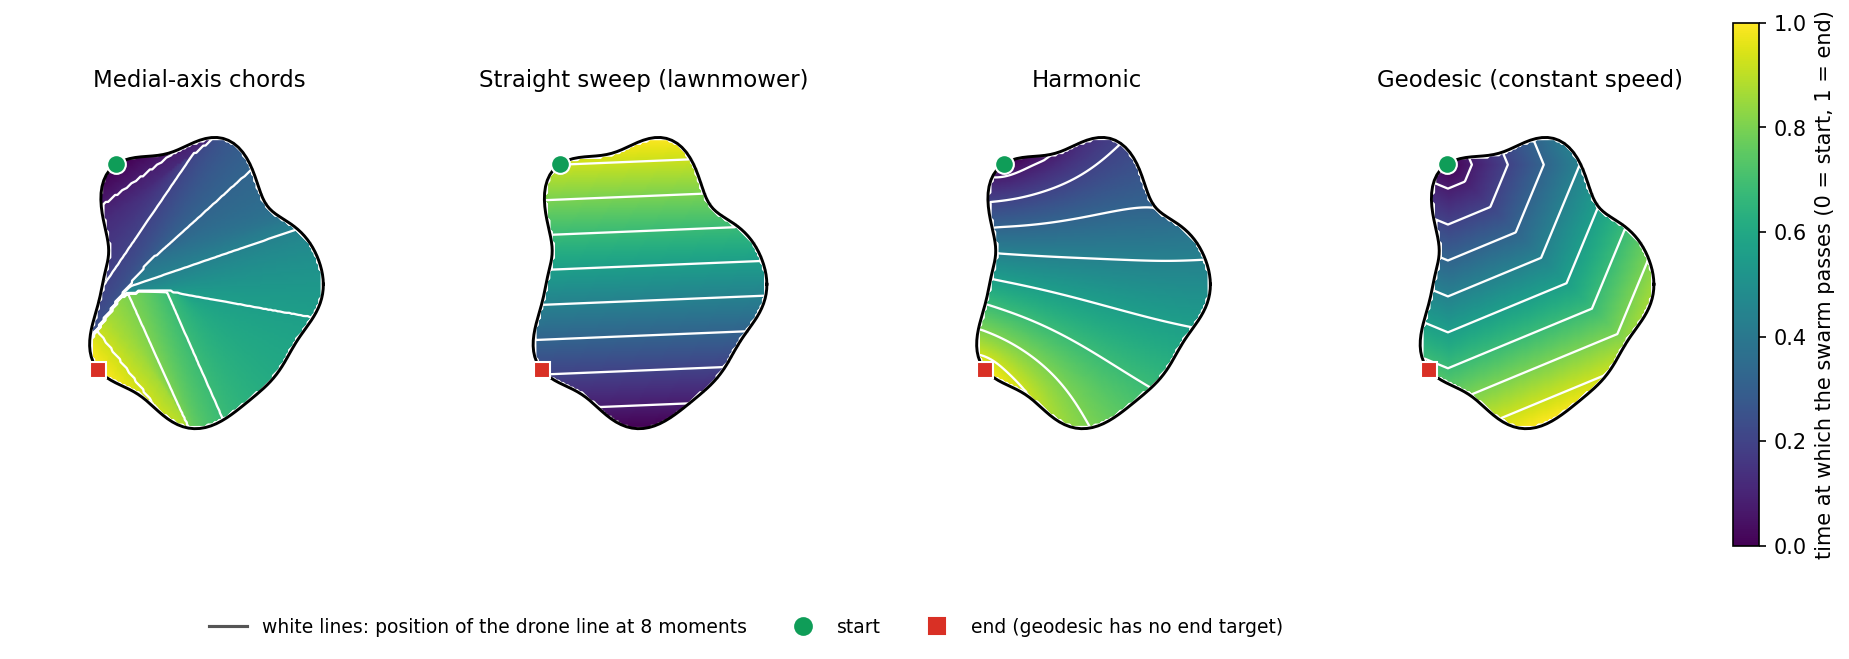
\includegraphics[width=\textwidth]{figures/fig3_sweeps.png}
  \caption{The four time maps on the same field. Colour shows when the swarm passes each point (dark = early, yellow = late). White lines show the position of the drone line at 8 moments. Green circle: start. Red square: end.}
  \label{fig:sweeps}
\end{figure}

\subsection{The four planners}

\paragraph{Medial-axis chords.} The \emph{medial axis} is the set of centres of the largest circles that fit inside the field \citep{blum1967}. We take its longest branch (the \emph{trunk}) and sweep with the chord perpendicular to it. This is the closest relative of the centre line of Section~2. However, the medial axis is equally far from both walls, which is \textbf{not} the same as cutting the chord in half. The two coincide only where the field is locally mirror-symmetric about the trunk. The average midpoint offset is 0.0 on an ellipse but 10 to 18 units on a star, a neck or a random blob. The chords also fold wherever \eqref{eq:nofold} fails.

\paragraph{Straight sweep (lawnmower).} $T$ is the position along the field's longest direction (its principal axis), so the drone line is always straight. This is the continuous version of a back-and-forth survey \citep{choset1998}. Every drone moves at the same speed, but the line splits at every dent in the boundary.

\paragraph{Harmonic.} Set $T=0$ at the start and $T=1$ at the end. In between, choose $T$ to minimise the energy $\int_\Omega|\nabla T|^2\,\dd x$, which is the smoothest way to go from 0 to 1. The Euler--Lagrange equation of this energy is Laplace's equation,
\begin{equation}
\Delta T = 0 .
\label{eq:laplace}
\end{equation}
By the maximum principle, a harmonic map has no peaks or pits inside the field. As a result, the drone line never closes into a loop and never folds back. Harmonic maps are already used for robot navigation \citep{connolly1990}. Minimising $\int|\nabla T|^p$ for other powers $p$ gives a family of related planners. As $p\to1$ this minimises the total length in \eqref{eq:coarea}, and as $p\to\infty$ it minimises the single longest drone line \citep{aronsson1967}.

\paragraph{Geodesic (constant speed).} $T$ is the shortest walking distance from the start, going around obstacles. It is the minimum value of the Lagrangian $\int|\dot x|\,\dd t$ over paths from the start, and it satisfies the eikonal equation \citep{sethian1999}
\begin{equation}
|\nabla T| = \text{constant},
\label{eq:eikonal}
\end{equation}
so the drone line advances at the same speed everywhere. Behind corners the line forms sharp kinks and splits. If the walking distance is measured from the \emph{whole} boundary instead, its kinks trace out exactly the medial axis; this is the ``grassfire'' picture of the medial axis \citep{blum1967,kimia1995}.

\subsection{How each map is computed}

The field is rasterised on a $200\times200$ grid.
\begin{itemize}
  \item \textbf{Medial axis.} We sample the boundary every 1 unit and compute the Voronoi diagram of the samples. The Voronoi edges inside the field approximate the medial axis \citep{brandt1992}. Short side branches caused by small bumps are removed \citep{ogniewicz1995}. The longest remaining path is the trunk, and its two ends define the start and end of the sweep for all planners.
  \item \textbf{Harmonic.} We solve the standard 5-point discrete Laplace equation with a sparse direct solver \citep{virtanen2020}.
  \item \textbf{Geodesic.} Shortest paths on the grid are computed by fast marching \citep{sethian1996}, as implemented in scikit-image \citep{vanderwalt2014}.
  \item \textbf{Drone-line positions.} We extract the level lines $T=t$ at 90 moments using marching squares \citep{lorensen1987}.
\end{itemize}

%==========================================================================
\section{From a time map to drones, paths and altitudes}
%==========================================================================

\begin{figure}[ht]
  \centering
  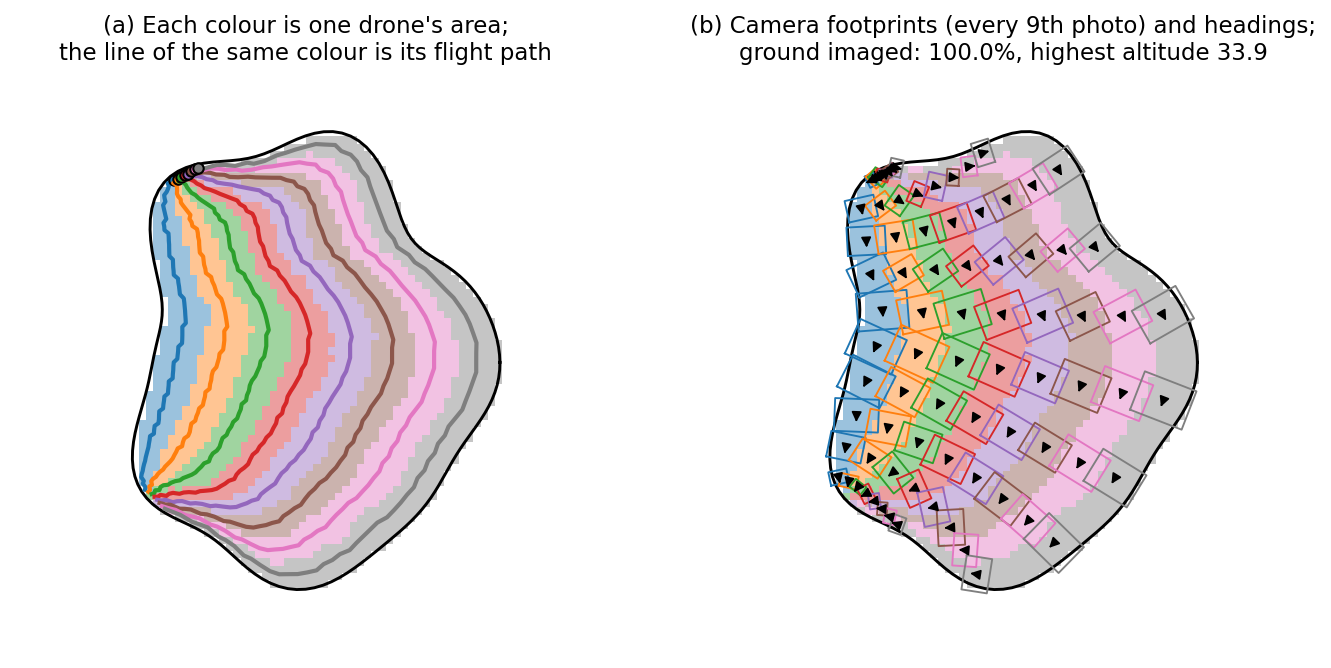
\includegraphics[width=\textwidth]{figures/fig4_drones.png}
  \caption{The harmonic plan with 8 drones. (a) The field divided among the drones (colours), with each drone's flight path. (b) Camera footprints for every 9th photo, with heading arrows. The whole field is photographed.}
  \label{fig:drones}
\end{figure}

\subsection{Splitting the field among the drones}

At each moment, the drone line is measured from one end to the other and scaled to run from 0 to 1. Drone $i$ is responsible for the part between $i/N$ and $(i+1)/N$, and flies along its middle at $(i+\tfrac12)/N$. Each point of the field belongs to the drone whose part passed over it. This divides the field into $N$ areas (Figure~\ref{fig:drones}a). When the line has split, a drone may have to hop from one piece to another; we call these hops \emph{transit jumps}.

\subsection{Choosing the altitudes}

At each photo position we know where the drone is and which way it is heading. Every point of the drone's area must lie inside some photo. Take a point at distance $\alpha$ ahead of or behind the nearest photo position, and $\beta$ to the side of it. The drone must then fly at an altitude of at least
\begin{equation}
h \;\ge\; \max\!\left(\frac{|\beta|}{\tan(\HFOV/2)},\;
\frac{|\alpha| - \tfrac12\,(\text{distance between photos})}{\tan(\VFOV/2)}\right).
\label{eq:altitude}
\end{equation}
At each photo position we take the largest requirement over all its points and add a 10\% overlap margin.

\subsection{Checking coverage and fixing gaps}

Next, we mark every grid cell that actually lies inside a photo. Extra photos are placed densely between positions, using the lower of the two neighbouring altitudes so that the check errs on the safe side. If any cell is missed, the drone responsible for it climbs slightly near that spot, and the check is repeated.

\begin{proposition}[Coverage can always be completed]
Flying higher never reduces coverage. Hence every correction only adds coverage, and at a high enough altitude every footprint contains the whole field.
\end{proposition}
\begin{proof}
A footprint is a rectangle that grows with $h$, so raising $h$ enlarges every photo, and therefore the union of all photos.
\end{proof}

In all our experiments every gap was closed within \textbf{two rounds}.

%==========================================================================
\section{Results}
%==========================================================================

The setup is 12 drones, $\HFOV=70^\circ$, $\VFOV=55^\circ$ and a 10\% overlap margin. The fields are an ellipse, a five-pointed star, a C-shaped bend, a field with a narrow neck, and a random blob. All four planners photographed \textbf{100\%} of every field. Altitudes are in canvas units; to convert to metres, multiply by the field width in metres divided by 600.

\begin{table}[ht]
\centering
\caption{Highest altitude needed. Lower is better; bold marks the best in each row.}
\label{tab:altitude}
\begin{tabular}{lrrrr}
\toprule
Field & Medial-axis & Lawnmower & Harmonic & Geodesic \\
\midrule
Ellipse     & 21.4  & \textbf{21.3} & \textbf{21.3} & 24.0  \\
Star        & 140.7 & 58.4          & \textbf{31.0} & 77.0  \\
C-bend      & 31.8  & 55.9          & \textbf{15.0} & 23.8  \\
Narrow neck & 93.5  & 84.1          & \textbf{21.1} & 159.2 \\
Blob        & 27.9  & 28.1          & \textbf{24.9} & 79.1  \\
\bottomrule
\end{tabular}
\end{table}

\begin{table}[ht]
\centering
\caption{Workload balance: smallest drone area divided by largest drone area (1 means perfectly equal). The last column shows how often medial-axis chords fold over.}
\label{tab:balance}
\begin{tabular}{lrrrrr}
\toprule
Field & Medial-axis & Lawnmower & Harmonic & Geodesic & Medial-axis folds \\
\midrule
Ellipse     & \textbf{0.94} & 0.81          & 0.79 & 0.86          & 0\%  \\
Star        & 0.12          & 0.80          & 0.41 & \textbf{0.81} & 23\% \\
C-bend      & 0.64          & \textbf{0.73} & 0.48 & \textbf{0.73} & 0\%  \\
Narrow neck & 0.16          & \textbf{0.85} & 0.32 & \textbf{0.85} & 42\% \\
Blob        & 0.16          & \textbf{0.87} & 0.39 & 0.84          & 52\% \\
\bottomrule
\end{tabular}
\end{table}

\paragraph{What the tables show.}
\begin{itemize}
  \item \textbf{Harmonic needs the lowest altitude on every field.} It minimises an energy that penalises long, stretched drone lines \eqref{eq:coarea}, and its line never folds. The drawback is uneven workload. The line bunches up in narrow parts and stretches in wide ones, so some drones cover far more ground than others.
  \item \textbf{Lawnmower and geodesic share the work most evenly,} because their lines move uniformly. However, both split around dents, and the geodesic line needs a very high altitude where it kinks (159 at the neck).
  \item \textbf{Medial-axis chords only work well on simple, tube-like fields.} Elsewhere the chords fold (Table~\ref{tab:balance}) and do not bisect.
\end{itemize}

\paragraph{Recommendation.} Use the harmonic plan when altitude is the main limit, for example because of camera resolution or regulations. Use the lawnmower or geodesic plan when battery life and an even workload matter more.

Computing all four plans takes 3--6\,s in Python and 0.8--2.3\,s in the browser demo.

%==========================================================================
\section{Checking the mathematics}
%==========================================================================

Every equation above was checked numerically with \texttt{paper/verify\_derivations.py}.

\begin{table}[ht]
\centering
\caption{Numerical checks of the equations.}
\begin{tabular}{p{9.2cm}cl}
\toprule
What is checked & Equation & Error found \\
\midrule
Wall-distance derivative w.r.t.\ position, 200 random chords in an ellipse & \eqref{eq:hit} & $4\times10^{-8}$ \\
Wall-distance derivative w.r.t.\ chord angle & \eqref{eq:hit} & $8\times10^{-8}$ \\
Euler--Lagrange equation splits as claimed (along-the-line part holds automatically) & \eqref{eq:el} & $3\times10^{-9}$ \\
Traced chord stays perpendicular to the motion of its midpoint & \eqref{eq:pair} & $8\times10^{-15}$ \\
Harmonic map satisfies the discrete Laplace equation & \eqref{eq:laplace} & $3\times10^{-15}$ \\
Harmonic map has the lowest energy (small changes only raise it) & \eqref{eq:laplace} & confirmed \\
Geodesic map moves at constant speed & \eqref{eq:eikonal} & confirmed \\
\bottomrule
\end{tabular}
\end{table}

The test suite \texttt{swarm\_lab/test\_medial.py} also checks that every planner gives each drone an area and photographs 100\% of the field.

%==========================================================================
\section{How to take the equations further}
%==========================================================================

\begin{enumerate}
  \item \textbf{Find the best exact centre line where one exists.} Trace \eqref{eq:pair}--\eqref{eq:start} from many starting points, keep the traces that reach the far side, and choose the start with the lowest cost \eqref{eq:search}. Check that every chord hits the \emph{nearest} wall, because in a non-convex field a traced chord can pass behind a bump. Chords that are perpendicular to the boundary at both ends are good places to begin the search.
  \item \textbf{Solve the curvature equation \eqref{eq:el} as a boundary-value problem} when an optimal line is wanted without the exact bisection requirement. Suitable solvers are collocation \citep{kierzenka2001}, available as \texttt{scipy.integrate.solve\_bvp}, and multiple shooting \citep{ascher1995}. Start from an easy shape such as an ellipse, morph it gradually into the real field, and re-solve at each step (numerical continuation, \citealp{allgower2003}). Watch the stiffness $f+f_{\theta\theta}$: wherever it turns negative, the line will want a corner.
  \item \textbf{Smooth out the wall jumps.} Replace ``nearest wall'' with a soft minimum over all walls, and sharpen it gradually. Alternatively, pose the whole problem as an optimisation and solve it with an interior-point method \citep{wachter2006} via CasADi \citep{andersson2019}. Pontryagin's maximum principle \citep{pontryagin1962,bryson1975} gives the same equations as \eqref{eq:constrained} and can also handle drone turning limits.
  \item \textbf{Minimise the worst altitude directly.} The harmonic map minimises an \emph{average}. To minimise the \emph{longest} drone line instead, minimise $\int|\nabla T|^p$ with increasing $p$ \citep{aronsson1967,chambers2009}.
  \item \textbf{Balance the harmonic plan's workload} by solving $\nabla\cdot\bigl(a(x)\nabla T\bigr)=0$ with a weight $a(x)$ chosen to even out the speed of the line. This sits between the harmonic and geodesic planners.
  \item \textbf{Find the exact minimum altitude.} Since flying higher never reduces coverage (Proposition~2), the lowest uniform altitude scale that gives full coverage can be found by bisection.
  \item \textbf{Real flight.} Add limits on turning and climb rate, follow the terrain from an elevation model, and convert the plan to GPS coordinates for the autopilot.
\end{enumerate}

%==========================================================================
\section{Limitations}
%==========================================================================

\begin{itemize}
  \item Exact bisecting centre lines exist only in convex or nearly convex fields (Section~\ref{sec:tracing}). The time-map approach is necessary, not just convenient.
  \item The medial axis is computed from boundary samples. How aggressively side branches are pruned affects the medial-axis planner, and also the start and end points of all planners.
  \item Coverage is guaranteed on a $200\times200$ grid. Features smaller than one cell (3 units) are not resolved.
  \item Battery, wind and flight dynamics are not modelled.
  \item The browser demo smooths the medial trunk differently from the Python version and uses grid Dijkstra instead of fast marching. Its results are close to, but not identical with, the Python results.
\end{itemize}

%==========================================================================
\section*{Reproducing this report}
%==========================================================================

\begin{verbatim}
py -m pip install -r swarm_lab/requirements.txt matplotlib
py paper/verify_derivations.py             # equation checks
py paper/figures.py                        # Figures 1-4
py paper/results.py                        # Tables 1-2
cd swarm_lab; py -m unittest test_medial   # coverage tests
\end{verbatim}

%==========================================================================
\begin{thebibliography}{99}
%==========================================================================

\bibitem[Allgower and Georg(2003)]{allgower2003}
E.~L. Allgower and K.~Georg.
\newblock \emph{Introduction to Numerical Continuation Methods}.
\newblock SIAM, 2003.

\bibitem[Andersson et~al.(2019)]{andersson2019}
J.~A.~E. Andersson, J.~Gillis, G.~Horn, J.~B. Rawlings, and M.~Diehl.
\newblock CasADi: a software framework for nonlinear optimization and optimal control.
\newblock \emph{Mathematical Programming Computation}, 11(1):1--36, 2019.

\bibitem[Aronsson(1967)]{aronsson1967}
G.~Aronsson.
\newblock Extension of functions satisfying Lipschitz conditions.
\newblock \emph{Arkiv f\"or Matematik}, 6:551--561, 1967.

\bibitem[Ascher et~al.(1995)]{ascher1995}
U.~M. Ascher, R.~M.~M. Mattheij, and R.~D. Russell.
\newblock \emph{Numerical Solution of Boundary Value Problems for Ordinary Differential Equations}.
\newblock SIAM, 1995.

\bibitem[Blum(1967)]{blum1967}
H.~Blum.
\newblock A transformation for extracting new descriptors of shape.
\newblock In W.~Wathen-Dunn, editor, \emph{Models for the Perception of Speech and Visual Form}, pages 362--380. MIT Press, 1967.

\bibitem[Brady and Asada(1984)]{brady1984}
M.~Brady and H.~Asada.
\newblock Smoothed local symmetries and their implementation.
\newblock \emph{The International Journal of Robotics Research}, 3(3):36--61, 1984.

\bibitem[Brandt and Algazi(1992)]{brandt1992}
J.~W. Brandt and V.~R. Algazi.
\newblock Continuous skeleton computation by Voronoi diagram.
\newblock \emph{CVGIP: Image Understanding}, 55(3):329--338, 1992.

\bibitem[Bryson and Ho(1975)]{bryson1975}
A.~E. Bryson and Y.-C. Ho.
\newblock \emph{Applied Optimal Control}.
\newblock Hemisphere, 1975.

\bibitem[Cabreira et~al.(2019)]{cabreira2019}
T.~M. Cabreira, L.~B. Brisolara, and P.~R. Ferreira~Jr.
\newblock Survey on coverage path planning with unmanned aerial vehicles.
\newblock \emph{Drones}, 3(1):4, 2019.

\bibitem[Chambers and Letscher(2009)]{chambers2009}
E.~W. Chambers and D.~Letscher.
\newblock On the height of a homotopy.
\newblock In \emph{Proceedings of the 21st Canadian Conference on Computational Geometry}, pages 103--106, 2009.

\bibitem[Choset(2001)]{choset2001}
H.~Choset.
\newblock Coverage for robotics: a survey of recent results.
\newblock \emph{Annals of Mathematics and Artificial Intelligence}, 31:113--126, 2001.

\bibitem[Choset and Pignon(1998)]{choset1998}
H.~Choset and P.~Pignon.
\newblock Coverage path planning: the boustrophedon cellular decomposition.
\newblock In \emph{Field and Service Robotics}, pages 203--209. Springer, 1998.

\bibitem[Connolly et~al.(1990)]{connolly1990}
C.~I. Connolly, J.~B. Burns, and R.~Weiss.
\newblock Path planning using Laplace's equation.
\newblock In \emph{Proceedings of the IEEE International Conference on Robotics and Automation}, pages 2102--2106, 1990.

\bibitem[Cort\'es et~al.(2004)]{cortes2004}
J.~Cort\'es, S.~Mart\'{\i}nez, T.~Karata\c{s}, and F.~Bullo.
\newblock Coverage control for mobile sensing networks.
\newblock \emph{IEEE Transactions on Robotics and Automation}, 20(2):243--255, 2004.

\bibitem[Evans(2010)]{evans2010}
L.~C. Evans.
\newblock \emph{Partial Differential Equations}.
\newblock American Mathematical Society, 2nd edition, 2010.

\bibitem[Galceran and Carreras(2013)]{galceran2013}
E.~Galceran and M.~Carreras.
\newblock A survey on coverage path planning for robotics.
\newblock \emph{Robotics and Autonomous Systems}, 61(12):1258--1276, 2013.

\bibitem[Gelfand and Fomin(1963)]{gelfand1963}
I.~M. Gelfand and S.~V. Fomin.
\newblock \emph{Calculus of Variations}.
\newblock Prentice-Hall, 1963.

\bibitem[Gurtin(1993)]{gurtin1993}
M.~E. Gurtin.
\newblock \emph{Thermomechanics of Evolving Phase Boundaries in the Plane}.
\newblock Oxford University Press, 1993.

\bibitem[Hairer et~al.(1993)]{hairer1993}
E.~Hairer, S.~P. N{\o}rsett, and G.~Wanner.
\newblock \emph{Solving Ordinary Differential Equations I: Nonstiff Problems}.
\newblock Springer, 2nd edition, 1993.

\bibitem[Kierzenka and Shampine(2001)]{kierzenka2001}
J.~Kierzenka and L.~F. Shampine.
\newblock A BVP solver based on residual control and the MATLAB PSE.
\newblock \emph{ACM Transactions on Mathematical Software}, 27(3):299--316, 2001.

\bibitem[Kimia et~al.(1995)]{kimia1995}
B.~B. Kimia, A.~R. Tannenbaum, and S.~W. Zucker.
\newblock Shapes, shocks, and deformations I: the components of two-dimensional shape and the reaction-diffusion space.
\newblock \emph{International Journal of Computer Vision}, 15:189--224, 1995.

\bibitem[Leyton(1987)]{leyton1987}
M.~Leyton.
\newblock Symmetry-curvature duality.
\newblock \emph{Computer Vision, Graphics, and Image Processing}, 38(3):327--341, 1987.

\bibitem[Lorensen and Cline(1987)]{lorensen1987}
W.~E. Lorensen and H.~E. Cline.
\newblock Marching cubes: a high resolution 3D surface construction algorithm.
\newblock \emph{ACM SIGGRAPH Computer Graphics}, 21(4):163--169, 1987.

\bibitem[Ogniewicz and K\"ubler(1995)]{ogniewicz1995}
R.~L. Ogniewicz and O.~K\"ubler.
\newblock Hierarchic Voronoi skeletons.
\newblock \emph{Pattern Recognition}, 28(3):343--359, 1995.

\bibitem[Pontryagin et~al.(1962)]{pontryagin1962}
L.~S. Pontryagin, V.~G. Boltyanskii, R.~V. Gamkrelidze, and E.~F. Mishchenko.
\newblock \emph{The Mathematical Theory of Optimal Processes}.
\newblock Interscience, 1962.

\bibitem[Sethian(1996)]{sethian1996}
J.~A. Sethian.
\newblock A fast marching level set method for monotonically advancing fronts.
\newblock \emph{Proceedings of the National Academy of Sciences}, 93(4):1591--1595, 1996.

\bibitem[Sethian(1999)]{sethian1999}
J.~A. Sethian.
\newblock \emph{Level Set Methods and Fast Marching Methods}.
\newblock Cambridge University Press, 2nd edition, 1999.

\bibitem[Taylor(1978)]{taylor1978}
J.~E. Taylor.
\newblock Crystalline variational problems.
\newblock \emph{Bulletin of the American Mathematical Society}, 84(4):568--588, 1978.

\bibitem[van~der Walt et~al.(2014)]{vanderwalt2014}
S.~van~der Walt, J.~L. Sch\"onberger, J.~Nunez-Iglesias, F.~Boulogne, J.~D. Warner, N.~Yager, E.~Gouillart, T.~Yu, and the scikit-image contributors.
\newblock scikit-image: image processing in Python.
\newblock \emph{PeerJ}, 2:e453, 2014.

\bibitem[Virtanen et~al.(2020)]{virtanen2020}
P.~Virtanen et~al.
\newblock SciPy 1.0: fundamental algorithms for scientific computing in Python.
\newblock \emph{Nature Methods}, 17:261--272, 2020.

\bibitem[W\"achter and Biegler(2006)]{wachter2006}
A.~W\"achter and L.~T. Biegler.
\newblock On the implementation of an interior-point filter line-search algorithm for large-scale nonlinear programming.
\newblock \emph{Mathematical Programming}, 106(1):25--57, 2006.

\end{thebibliography}

\end{document}
